\documentclass[cjjs]{ipart}
\RequirePackage{hyperref}
\usepackage{graphicx}
\usepackage{float}


\startlocaldefs
\theoremstyle{plain}
\newtheorem{thm}{Theorem}[section]
\def\SM#1#2{\sum_{#1\in #2}}
\def\FL#1{\left\lfloor #1 \right\rfloor}
\def\FR#1#2{{\frac{#1}{#2}}}
\endlocaldefs


\pubyear{2025}
\volume{2}
\issue{1}
\firstpage{175}
\lastpage{199}
\arxiv{0000.0000}

\begin{document}

\begin{frontmatter}

\title[Running title]
{Optimizing Dart Throwing Strategies for the Elderly Based on Markov Decision Process*}

\thankstext{T1}{Award: 2024 S.-T. Yau High School Science Award (YHSA)}

\thankstext{t2}{Acknowledgment for contributions or funding related to Yunshan Gong.}

\begin{aug}
    \author{\fnms{Yunshan} \snm{Gong}\thanksref{t2}\ead[label=e1]{Yunshan.gong@outlook.com}}
    \address{Beijing No.101 High School,\\
             China\\
             \printead{e1}}
    
\end{aug}

\received{\sday{} \smonth{} \syear{2024}}

\begin{abstract}
\noindent
Dart throwing can potentially enhance the quality of life for the elderly. However, lack of effective throwing strategy guidance, excessively difficult competitions, and insufficient training due to physical limitations can hinder their experience and participation in this beneficial activity. To address the issues, this paper innovatively formalizes the dart throwing process as a Markov Decision Process (MDP). By leveraging this theoretical framework, I design a scientific dart throwing strategy aimed at lowering the learning barrier. Furthermore, this research proposes two simplified dart competition rules tailored to the elderly, with the objective of enhancing the inclusivity of the sport. Additionally, I have developed an efficient and adaptable training program designed to assist the elderly in achieving optimal training outcomes within limited timeframes.
\end{abstract}

\begin{keyword}
\kwd{Markov Decision Process}
\kwd{Healthy Aging}
\kwd{Dart Sports}
\kwd{Nearest Neighbor Method}
\end{keyword}

\end{frontmatter}
    
\section{Introduction}

In 2022, the National Health Commission of China and 15 related departments jointly issued the "14th Five-Year Plan for Healthy Aging" [1], which pointed out that the health status of the elderly in China is not optimistic. Age-related decline in cognitive, motor, and sensory functions, as well as nutritional and psychological health problems, are becoming increasingly prominent. Therefore, the plan encourages the elderly to engage in scientific exercise, recognizing that improving their fitness experience is an effective way to enhance their quality of life. On the other hand, academic research (Crombie et al., 2004) [2] indicates that older adults often have negative experiences when trying to engage in fitness activities. This is due to factors such as a lack of interest-driven guidance, physical limitations, and fear of injury, making it difficult for them to persist through the initial stages and leading them to abandon beneficial exercise opportunities.

Exercise programs suitable for the elderly should be both enjoyable and appropriately challenging, and darts align well with these criteria. Darts have a long history, originating in 15th-century England and introduced to China in the 1980s. In recent years, numerous studies have demonstrated the significant health benefits of darts for older adults. Notably, TAKEDA et al. [3] showed that regular darts training can significantly improve memory in older individuals, which is crucial for their well-being in later life. Chinese scholar (Xiao Xin, 2013) has also conducted relevant research [4][5], finding that darts are beneficial for both coordination and balance in older adults. These findings support the conclusion that darts are a highly suitable fitness activity for the elderly population.

China has a rich tradition of fitness activities, such as "Touhu" (arrow throwing) and "Sheli" (archery), as well as a profound understanding of strategic planning and game theory. Based on this background, this research leveraged the school's darts society as a base, organizing members to conduct darts training activities for the elderly in their homes and communities. Through these activities, interviews, surveys, and data collection were carried out. Building upon this foundation, we established a mathematical model tailored to the characteristics of older adults. By solving this model, we deduced three strategies suitable for elderly individuals to participate in fitness activities, helping them smoothly transition through the initial stages of darts, maintain consistent exercise, and reap the associated joy and health benefits.


\section{Related Work}
In recent years, with the growing global popularity of darts, academic research on dart throwing strategies has deepened. Ryan J. Tibshirani et al. investigated dart throwing strategies based on statistical methods. They employed bivariate normal and skew-normal distributions to establish a dart throwing model, utilizing the standard deviation of the normal distribution to characterize a player's skill level. The Expectation-Maximization (EM) algorithm was applied to estimate the standard deviations of dart throws in both the X and Y directions [6]. Their findings, based on the results of 100 throws, indicated that this method can accurately estimate the true skill level of a dart player, which can assist players in achieving higher scores in a single round.

Darts is a competitive sport involving two or more players, prompting researchers to investigate game strategies from a game theory perspective. Haugh and Wang conducted an in-depth data analysis on a dataset of 16 top professional dart players from the 2019 season [7]. This study utilized the dataset to construct models that fit player skills, subsequently employing these models to simulate the dynamic zero-sum game (ZSG) process of actual matches between dart players. Their experiments demonstrated that employing a game strategy based on this ZSG model, which involves strategic play considering both the player's own skill level and the opponent's score, can increase the probability of winning by approximately 2\% to 3\%.

Investigations from a sports engineering perspective have also yielded compelling results. James et al. examined the influence of dart flight trajectory on performance outcomes [8]. Utilizing high-speed video capture, they recorded the trajectories of 225 dart throws by 19 amateur players. Their analysis revealed that the pitch angle of the dart during flight oscillates in a manner akin to damped harmonic motion.  Furthermore, the study found a strong correlation between this oscillation frequency and launch speed, while the characteristic wavelength and damping ratio were independent of launch speed. Notably, the measured oscillation wavelength (2.16 m) closely approximated the regulated throwing distance (2.37 m). The authors suggest "tuning" the dart throwing distance to the wavelength, allowing the dart to undergo one complete oscillation before striking the dartboard. This study employed classical dynamic stability analysis to model dart flight, demonstrating strong agreement between experimental observations and theoretical predictions.

While previous research has primarily focused on dart enthusiasts or high-level players, the elderly participate in darts with distinct motivations and characteristics. Their objectives are not centered on winning competitions or earning prize money, but rather on physical and mental fitness, and enhancing their quality of life. This presents unique challenges, such as lower accuracy, limited physical stamina and energy, and reduced training time. Therefore, it is essential to develop models specifically tailored to the needs and capabilities of older adults, and to propose strategies that are suitable for this demographic.


\section{Dart Throwing Strategy Modeling}

\subsection{Rules of Dart Games}
A standard dartboard comprises six concentric circles, uniformly divided into 20 radial sectors. Each sector is assigned a specific score value, as illustrated below.


\begin{figure}
        \centering
        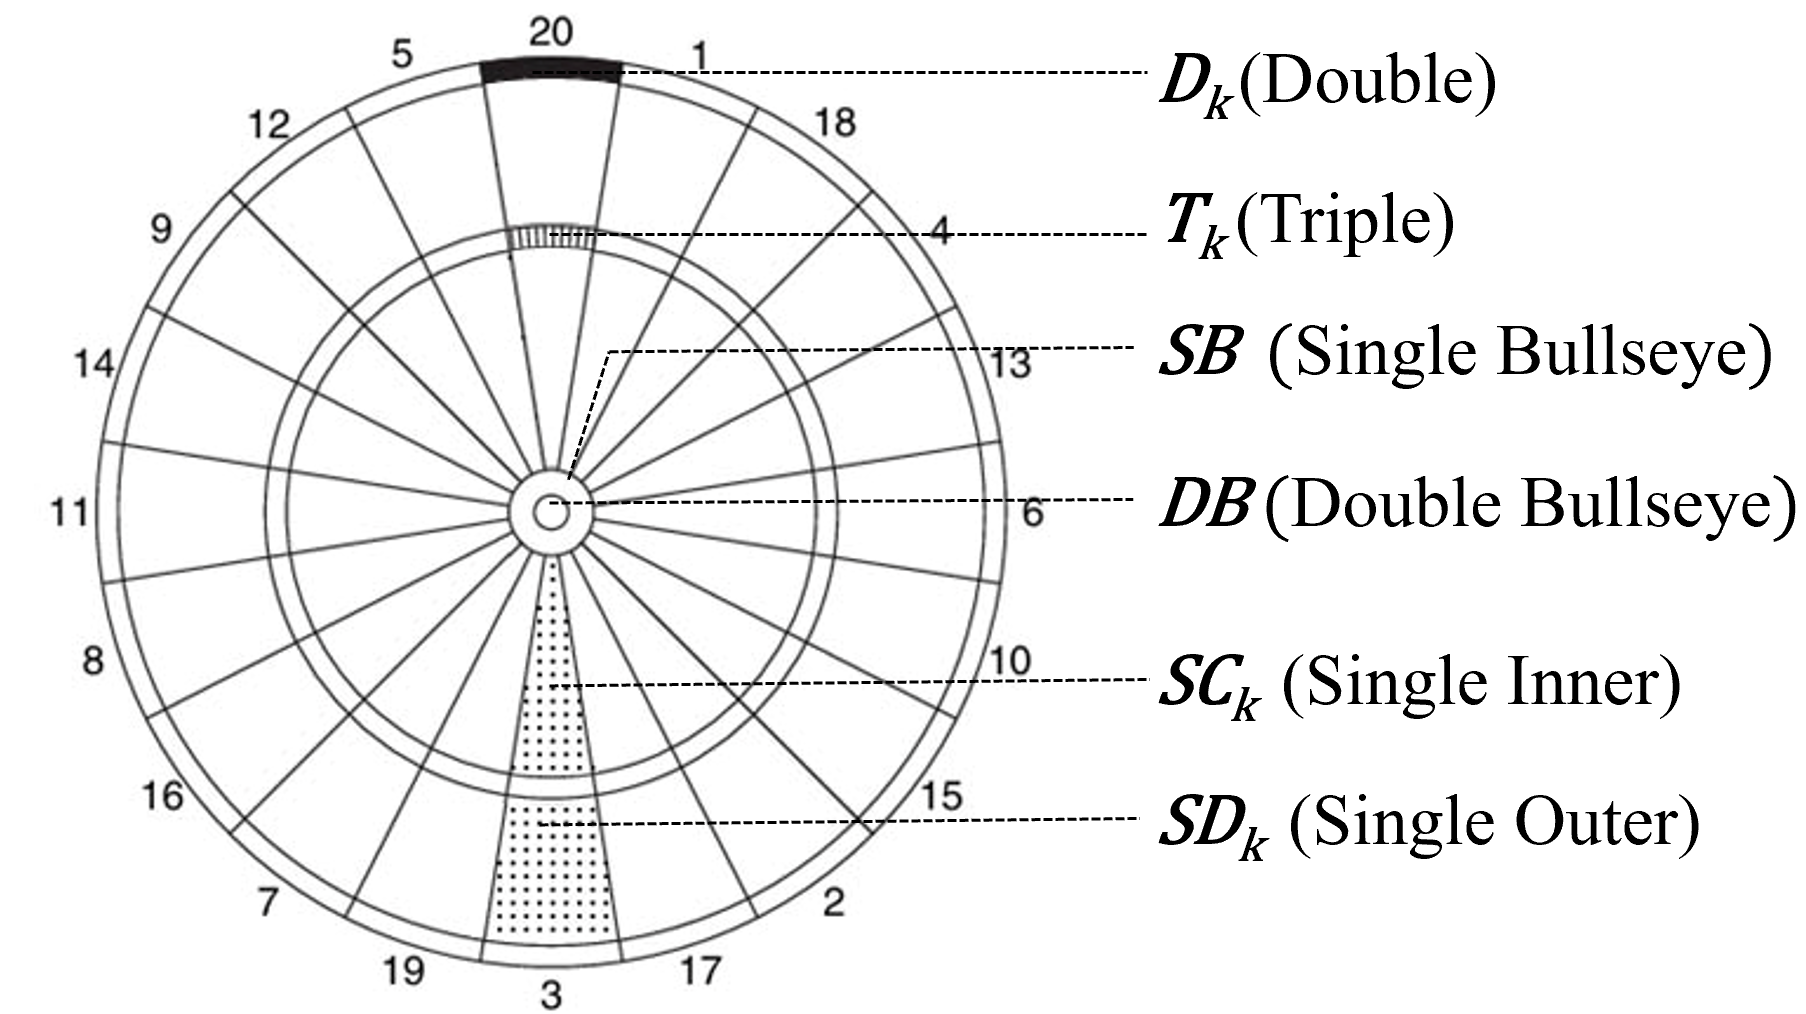
\includegraphics[width=0.60\textwidth]{1.png}
        \caption{Dartboard and its respective scoring zones}
        \label{fig:enter-label}
     \label{fig:dartboard}
\end{figure}


The dartboard encompasses 82 distinct scoring zones, each with a corresponding point value. Any area outside the board is assigned a score of zero. The symbols and scores for each zone are detailed in Table 1, where k represents the score value of the outermost ring $\begin{aligned}k \in \{1, 2, \dots, 20\}.\end{aligned}$
\begin{table}[h]
    \centering
    \begin{tabular}{|c|c|c|c|}
        \hline
        Name & Description & Symbol & Score \\
        \hline
        Double Bullseye & The innermost circle at the center. & DB & 50 \\
        \hline
        Single Bullseye & The annular ring surrounding DB. & SB & 25 \\
        \hline
        Single Inner & The 20 pie-shaped sectors encircling SB. & \( SC_k \) & \( k \times 1 \) \\
        \hline
        Triple & The 20 annular sectors surrounding \( SC_k \). & \( T_k \) & \( k \times 3 \) \\
        \hline
        Single Outer & The 20 annular sectors surrounding \( T_k \). & \( SD_k \) & \( k \times 1 \) \\
        \hline
        Double & The 20 annular sectors surrounding \( SD_k \). & \( D_k \) & \( k \times 2 \) \\
        \hline
    \end{tabular}
    \caption{\textbf{Symbols and scores for the dartboard and its respective scoring zones}}
\end{table}

Furthermore, we denote the set of target locations as:

\[
\text{Target} = \{ \text{DB}, \text{SB}, \text{SC}_k, \text{SD}_k, \text{T}_k, \text{D}_k \}, k \in \{1, 2, \dots, 20\}
\]


We also denote the score obtained by hitting \( X \) as \( \text{Score}(X) \), where \( X \in \text{Target} \).  
For example, 
$\text{Score}(T_3) = 3 \times 3 = 9, \quad \text{Score}(DB) = 50.$
The 501 game is the most prevalent in the sport of darts. While regional variations exist, this study adopts the four most fundamental rules of the 501 game, outlined in Table~\ref{tab:rules}.
\begin{table}[h]
    \centering
    \begin{tabular}{|c|c|p{10cm}|}
        \hline
        No. & Rule Name & Contents of the Rule \\
        \hline
        1 & Scoring Rule & Each player begins with a score of 501. A player's score decreases with each successful throw. The first player to reach a score of exactly zero wins the game. \\
        \hline
        2 & Double Out Rule & The final dart thrown must land in the doubles ring (i.e., hit a \( D_k \)) to conclude the game. \\
        \hline
        3 & Bust Rule & If a dart hits outside of the board, or if the resulting score would be 1, 0 (but does not satisfy the "Double Out" rule), or negative, the player's score remains unchanged from before the throw. \\
        \hline
        4 & Alternate First Rule & The two players alternate who throws first in each round. \\
        \hline
     \end{tabular}
     \caption{\textbf{The fundamental rules of the 501 dart game.}}
     \label{tab:rules}
\end{table}


\subsection{Model and Mathematical Symbols}
The process of a dart player completing a 501 game can be regarded as a sequential decision-making process, with an initial state of 501 points. Before each throw, the player must select a suitable target based on their current score. The outcome of the throw exhibits inherent randomness due to the player's skill level. Once the dart lands, the player deducts the corresponding score and selects the next target for throwing, continuing this process until the remaining score reaches exactly zero in accordance with the rules outlined in Table 2.

\begin{figure}[h]
    \centering
    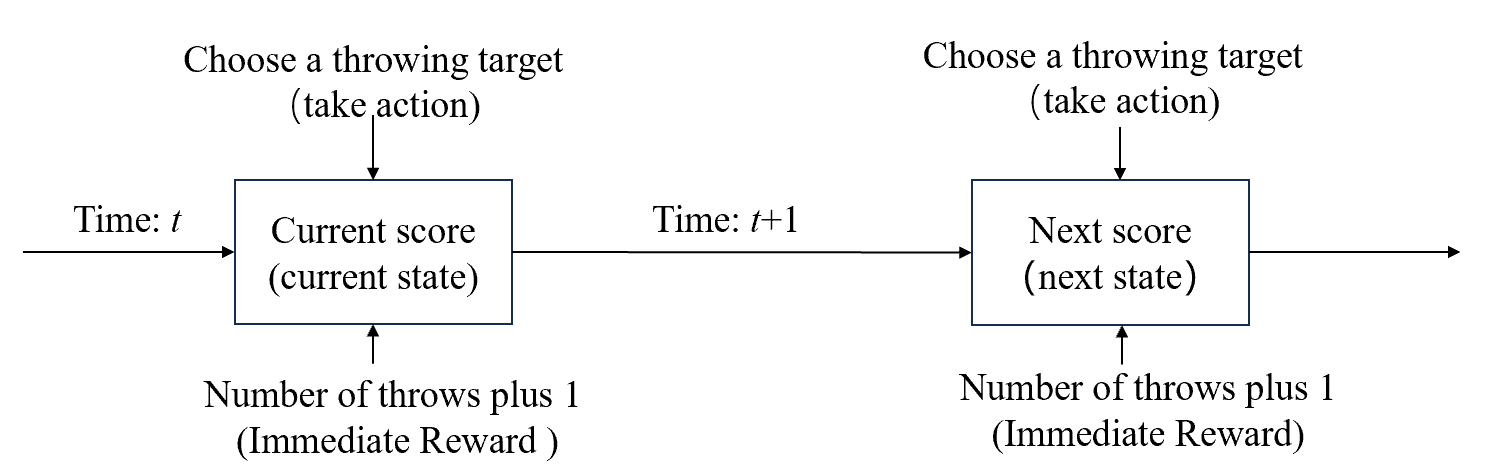
\includegraphics[width=0.60\textwidth]{2.png} 
    \caption{\textbf{Sequential decision-
making process in dart throwing}}
    \label{fig:dartboard}
\end{figure}

We model the process of a player's 501 Game using a Markov Decision Process (MDP), and it can be characterized by a quintuple:

\[
\text{Dart-MDP} = \left\{ T, S, A, p(s_{t+1} \mid s_t, a), r(s_t, a) \right\}
\]

Where:  

$T= \{ 0, 1, \cdots\}$ is the decision time point set, and the time point t at which a darts player chooses a target for throwing is the moment of decision. Considering that some players’ skills may be at very low levels and they are unable to complete the game, T in this context is an infinite set.

$S = \{501, 500, 499, \dots, 2, 0\}$ is the state space and represents the player's current remaining score. It is important to note that there is no state of "1" because of the "double out rule".

$A = \{ DB, SB, SC_k, SD_k, T_k, D_k \}$ is the action set, where $k \in \{ 1, 2,\cdots, 20 \}$. The action set consists of the 82 target positions on the dartboard, which correspond to the target set defined in Section 3.1.

$p(s_(t+1) s_t,a)$ is the transition probability. It refers to the probability of the system transitioning to a states$s_{t+1} \in S$ at the next decision moment after the player, in states$_t \in S$, takes an action $a \in A$(i.e., aiming at a specific position and throwing), and$\sum_{s_{t+1} \in S} p(s_{t+1} \mid s_t, a) = 1$.For example, if a player is in state $s_t = 300$ and takes an action $a = T_{20}$, meaning they aim at $a = T_{20}$and throw, they might hit $a = T_{20}$, ut they could also hit areas around, ut they could also hit areas around,such as $T_1, T_5, SC_5$,etc.Thus, the next state $s_{t+1}$ could be 240, 297, 285, 295, and so on.

$r(s_t,a)$is the immediate reward. According to the rules of the 501 games, when a player is in state $s_t$ and makes a throw a , the number of throws increases by one. Define
$r(s_t, a) := 1$,which acts as a counter in the subsequent optimization process.

When constructing the Dart-MDP model for a darts player, the set of decision time points T, state space S, action set A, and reward function $r(s_t, a)$are all fixed. The only unknown is the transition probability $p(s_{t+1} \mid s_t, a)$,which is determined by the player's dart skill. The following discusses how to calculate the transition probability.

\subsection{Solving the Transition Probability}

The transition probability $p (s_{t+1} \mid s_t, a)$ represents the probability that, when the player is in state $s_t \in S$ and takes an action $a\in A $(i.e., aims at a target a and throws), the system transitions to state $s_{t+1} \in S$ at the next decision time point. This can be expressed as the probability of the event that the player, aiming at $a \in A$ and throwing, achieves a score of$(s_t - s_{t+1})$.

\begin{equation}
p(s_{t+1} \mid s_t, a) = P(\text{target} = a, \text{score} = (s_t - s_{t+1})) \hspace{1cm} \tag{1}
\end{equation}

The scoring rule permits multiple hit locations to achieve the same score.

$$P(\text{target} = a, \text{score} = (s_t - s_{t+1})) =$$
 
\begin{equation}
\sum_{h \in \{z \mid \text{Score}(z) = (s_t - s_{t+1}) \}} P(\text{target} = a, \text{hit} = h) \tag{2}
\end{equation}

$P(\text{target} = a, \text{hit} = h)$represents the probability that a player aims at the $\text{target} = a$\and hits the region $\text{hit} = h$. Since darts can miss the board, $h \in A \cup \{ \text{MISSED} \}$
The score at a position z on the dartboard is denoted by $\text{Score}(z)$.

Using the method proposed by Ryan J.T. et al. [6], a player's skill level is characterized by the standard deviations $(\sigma_X, \sigma_Y)$ of two independent bivariate normal distributions in the X and Y directions. The probability of hitting a region $h = \text{hit}$ after aiming at the $\text{target} = a$ can be calculated using the integral formula of a bivariate normal distribution as follows:

\begin{equation}
P(\text{target}=a, \text{hit}=h) = \iint_h \frac{1}{2\pi \sigma_X \sigma_Y} \exp\left( -\frac{(x - \mu_{aX})^2}{2 \sigma_X^2} - \frac{(y - \mu_{aY})^2}{2 \sigma_Y^2} \right)\,dx\,dy \tag{3}
\end{equation}

Where:

$(\mu_{aX}, \mu_{aY})$ are the X- and Y-coordinates of the centroid of the target region.

$(\sigma_X, \sigma_Y)$ are the standard deviations reflecting the player's throwing accuracy in the $X-$ and $Y-$ directions. 

Combining equations (1), (2), and (3), we can derive the formula for calculating the formula for $p(s_{t+1} \mid s_t, a)$ as blow:

\[
p(s_{t+1} \mid s_t, a)=
\]

\begin{equation}
\sum_{h \in \{ z \mid \text{score}(z) = (s_t - s_{t+1}) \}} \iint_h \frac{1}{2 \pi \sigma_X \sigma_Y} \exp \left( - \frac{(x - \mu_{aX})^2}{2 \sigma_X^2} - \frac{(y - \mu_{aY})^2}{2 \sigma_Y^2} \right) \, dx\,dy \tag{4}
\end{equation}

Equation (4) is transformed into polar coordinates, thereby simplifying the double integral computation.
\[
p(s_{t+1} \mid s_t, a) =
\]

\begin{equation}
\sum_{h \in \{ z \mid \text{Score}(z) = (s_t - s_{t+1}) \}} \iint_h \frac{1}{2 \pi \sigma_X \sigma_Y} \exp \left( - \frac{(\rho \cos \theta - \mu_{aX})^2}{2 \sigma_X^2} - \frac{(\rho \sin \theta - \mu_{aY})^2}{2 \sigma_Y^2} \right) \rho \, d\rho \, d\theta\tag{5}
\end{equation}

The above derivation highlights that the standard deviations$(\sigma_X, \sigma_Y)$ of the bivariate normal distribution are critical determinants of the transition probability. The following section explores methods for estimating a player's skill level.

\subsection{Estimating Dart Throwing Accuracy}

Ryan J.T. and his colleagues utilized the Expectation-Maximization (EM) algorithm to estimate the standard deviations$(\sigma_X, \sigma_Y)$ for different dart players [6]. Smaller standard deviations indicate a higher skill level for the players. However, since elderly individuals often have limited physical stamina, it can be challenging to collect sufficient trial throw data to apply the EM algorithm. Therefore, in community practice, this study employs a nearest-neighbor estimation method (referred to as the "nearest-neighbor estimation method") to estimate the dart throwing accuracy of dart players.

The nearest neighbor estimation method is as follows: construct N virtual dart-throwing robots with varying accuracy levels (represented by standard deviations$(\sigma_X, \sigma_Y)$. The landing distribution of each robot's darts follows a bivariate normal distribution with distinct standard deviations. Utilizing equation (3) from the previous section, we can calculate the probability of each robot hitting various locations on the dartboard when aiming at different targets$\left( P(\text{target}=a, \text{hit}=h),\, a \in A, \, h \in A \cup \{\text{MISSED}\} \right)$. After completing the computation of the virtual robot throwing data, we calculate the similarity between the trial throw data of an older dart player and the simulated data of each robot. This allows us to identify the robot with the landing distribution most closely resembling that of the player. The standard deviations of this most similar robot in the X and Y directions are then adopted as the estimated standard deviations for the older player. Various distance metrics can be employed to calculate similarity, such as Euclidean distance, Manhattan distance, etc. In this study, we utilize Euclidean distance as the measure of similarity.

\begin{figure}[h]
    \centering
    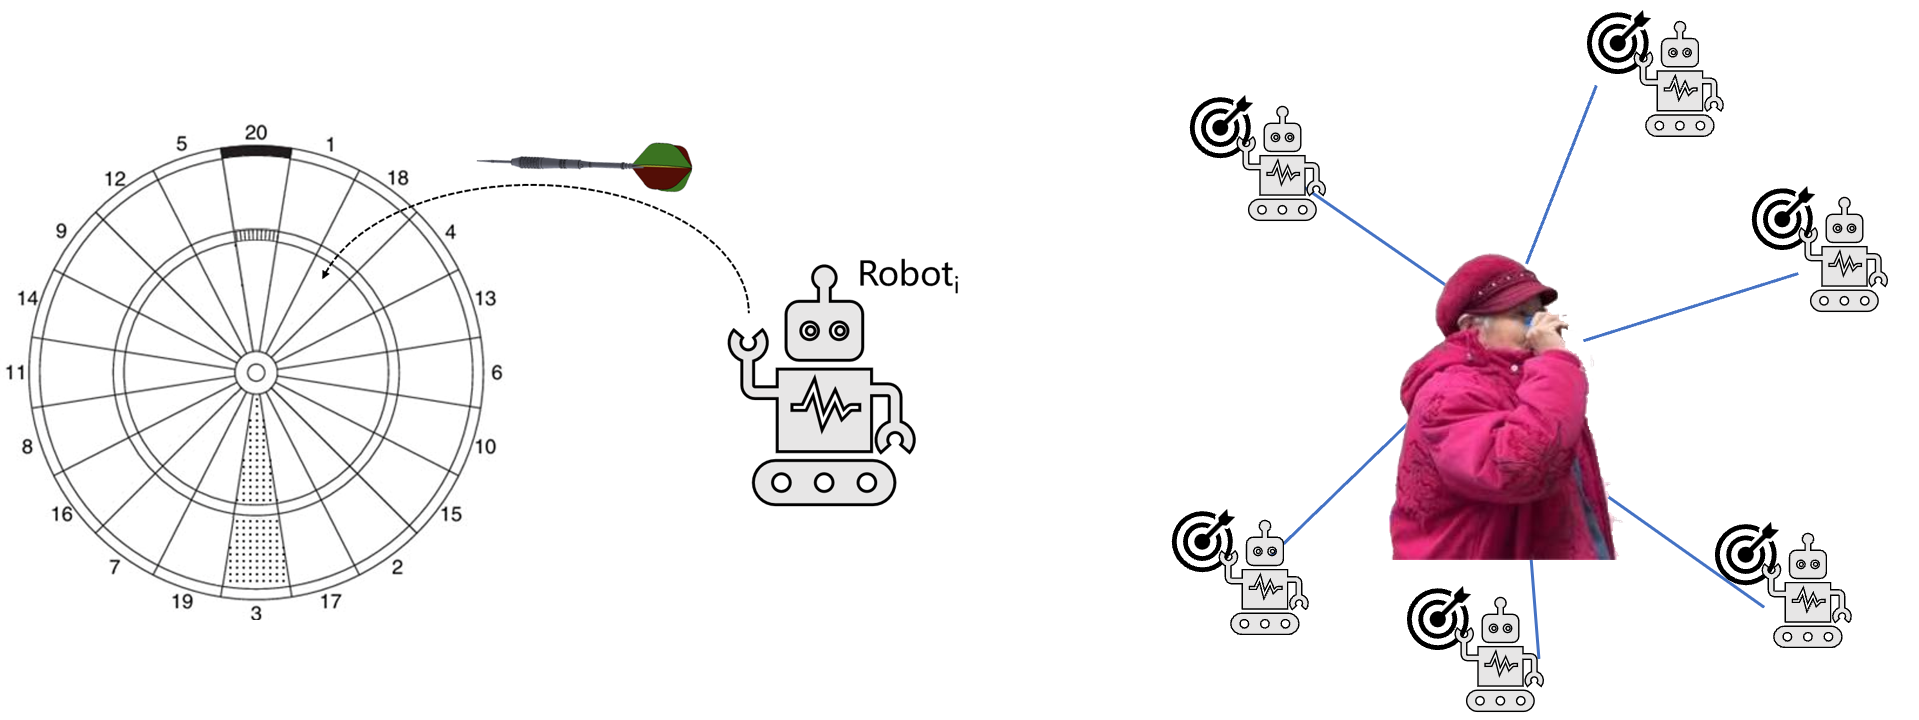
\includegraphics[width=0.60\textwidth]{3.png} 
    \caption{\textbf{Estimating Accuracy
of the Elderly Using the Nearest Neighbor Method}}
    \label{fig:dartboard}
\end{figure}


In the experiment, we construct N virtual robots for dart throwing. The two key parameters influencing a robot's skill level are the standard deviations in the X and Y directions. Both standard deviations begin at 0.1 centimeters and increase in increments of 0.1 centimeters up to 3.0 centimeters. Beyond 3.0 centimeters, the increment size changes to 0.2 centimeters, continuing up to 10 centimeters. This varying increment size is employed because high-skill players (with standard deviations less than 3.0 centimeters) require finer granularity in robot skill levels for accurate matching. Conversely, for players with standard deviations greater than 3 centimeters, a 0.2-centimeter increment is sufficient for reasonably accurate estimation. In this manner, a total of N=4225 robots with varying skill levels are constructed.

Dart throwing data were collected from the elderly by hosting dart throwing events within the neighborhoods, and the accuracy levels of four elderly players were estimated. To validate the accuracy of the method, the skill level of Michael Van Gerwen, the 2019 World Darts Champion, was also estimated, as shown in Figure 4.

\begin{figure}[h]
    \centering
    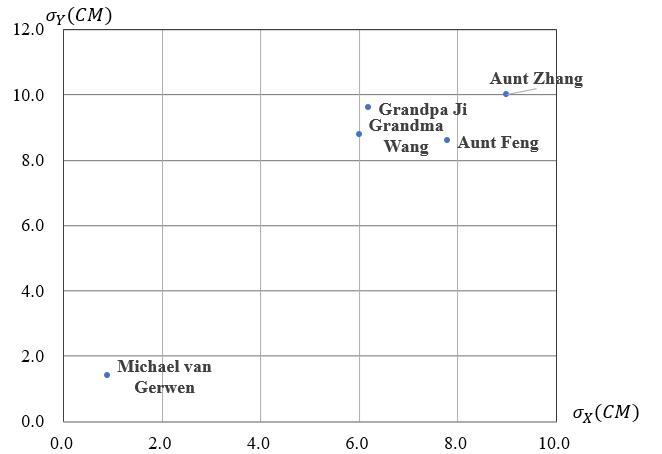
\includegraphics[width=0.60\textwidth]{4.png} 
    \caption{\textbf{Accuracy Estimation for Four Elderly Players and Wold Champion}}
    \label{fig:dartboard}
\end{figure}

The accuracy estimations for the five dart players show that world champion Michael van Gerwen exhibits exceptional skill, with a lateral standard deviation of 0.9 centimeters and a longitudinal standard deviation of 1.4 centimeters between his dart landing positions and the intended target.  A significant disparity in accuracy level is observed between the four elderly dart players and the world champion.  Furthermore, there is noticeable variation among the four older adults, with Grandma. Wang demonstrating a slight advantage over the others.

\section{Strategy Optimization}
\subsection{Dart Throwing Strategy Optimization}
In the 501 games, each player aims to complete the game with as few throws as possible, which can be expressed as solving:$\min \left( \sum r(s_t, a) \right)$. Let $E[s_t, a]$ note the expected minimum number of throws required for a player to complete the game when in state $s_t$,and taking action $a \in A$. Define:

\[
E_{\min}[s_t] := \min_{\alpha \in A} \big( E[s_t, a] \big)
\]

which represents the smallest expected number of throws across all actions in state $s_t$. If an action $a$ satisfies $E[s_t, a] = E_{\min}[s_t]$, it is called the optimal decision for state $s_t$.
\[
a_{s_t}^* \coloneqq \arg\min_{\alpha \in A} E[s_t, \alpha]
\]
The set of all optimal decisions across the entire state space S constitutes the optimal strategy of the player$\{ a_{s_t}^* \mid s_t \in S \}$.

Utilizing the state transition probabilities within the Dart-MDP model,we leverage dynamic programming to derive the optimal strategy. The first step is to illustrate the state transition diagram when the player is in state $s_t = i$, and aims at target $a$, as depicted in Figure 5.

\begin{figure}[h]
    \centering
    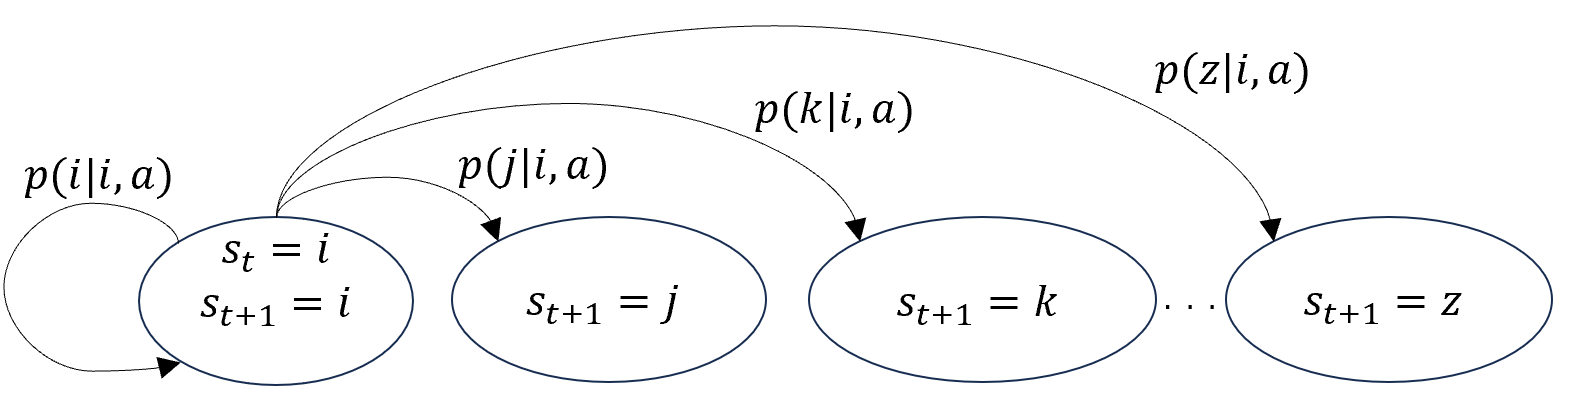
\includegraphics[width=0.60\textwidth]{5.png} 
    \caption{\textbf{State Transition Dia-
gram for a Player Aiming at Target a in State $st = i$}}
    \label{fig:dartboard}
\end{figure}

Applying the definition of mathematical expectation, we can get:

$$E[s_t \mid s_t = i, a] =$$

\begin{equation}
p(s_{t+1} = i \mid s_t = i, a) \left( 1 + E[s_t = i, a] \right) + \sum_{j \neq i, j \in S} p(s_{t+1} = j \mid s_t = i, a) \times E_{\min}[s_{t+1} = j] \tag{6}
\end{equation}

By reformulating Equation (6), the mathematical expectation of the minimum number of throws required for a player to complete the game when in state$s_t$ and taking action $a$ can be expressed as:

\begin{equation}
E[s_t = i, a] = \frac{p(s_{t+1} = i \mid s_t = i, a) + \sum_{j \neq i, j \in S} \left( p(s_{t+1} = j \mid s_t = i, a) \times E_{\min}[s_{t+1} = j] \right)}{1 - p(s_{t+1} = i \mid s_t = i, a)}
\tag{7}
\end{equation}

Following the principles of dynamic programming, we first calculate $E_{\min}[2]$. Subsequently, by iterating backwards, we compute the optimal decision for all states, thereby deriving the optimal strategy for the player.

To illustrate this process, consider a player with$(\sigma_X = 1.8, \sigma_Y = 2.2)$. Figure 4 depicts the state transition diagram when this player is in state $s_t = 2$ and takes different actions a to transition to the next state $s_{t+1} = 0$

\begin{figure}[h]
    \centering
    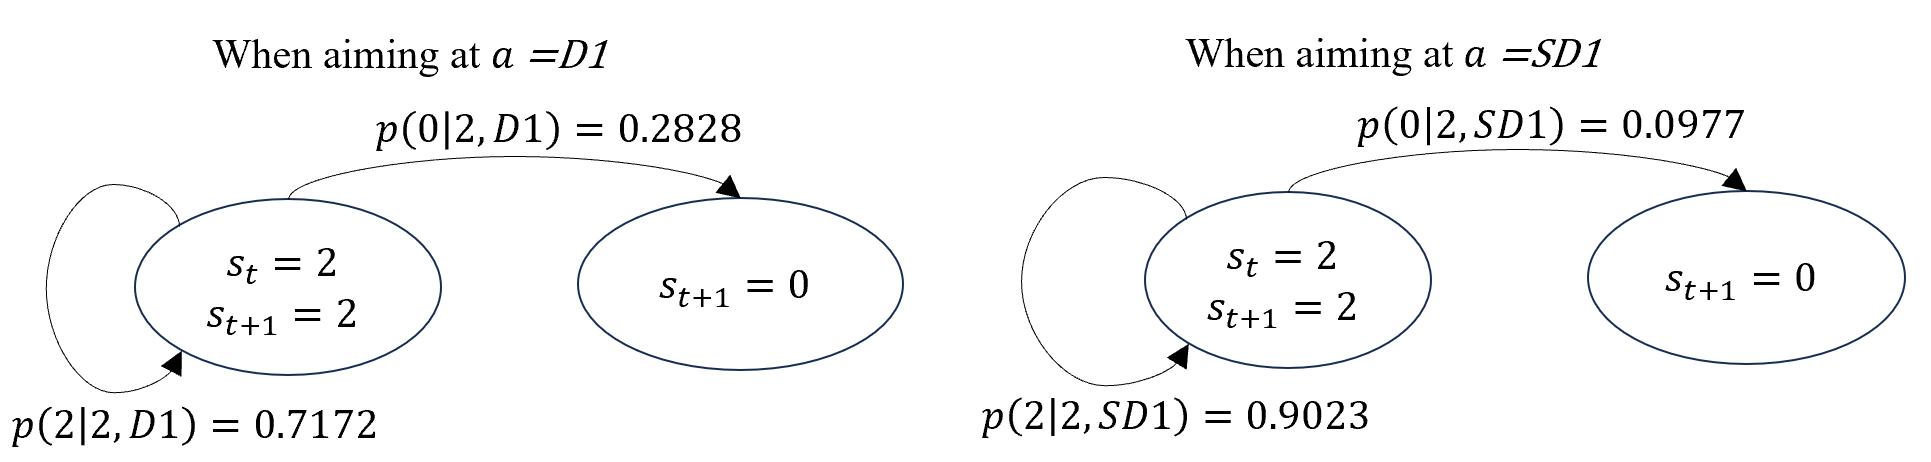
\includegraphics[width=0.60\textwidth]{6.png} 
    \caption{\textbf{Transition diagrams
for a player in state $st = 2$ aiming at different targets}}
    \label{fig:dartboard}
\end{figure}

From the state transition diagram above, the expected number of throws required to transition from $s_t = 2$ to $s_{t+1} =0$ is:

when aiming at $D1,E(2, D1) = 3.536$,

when aiming at $SD1,E(2, \text{SD1}) = 10.235$

After calculating the expected number of throws for all 82 targets, we find that is the optimal decision in state $s_t = 2$ for the player, and $E_{\min}(2) = E(2, \text{D1}) = 3.536$

\begin{figure}[h]
    \centering
    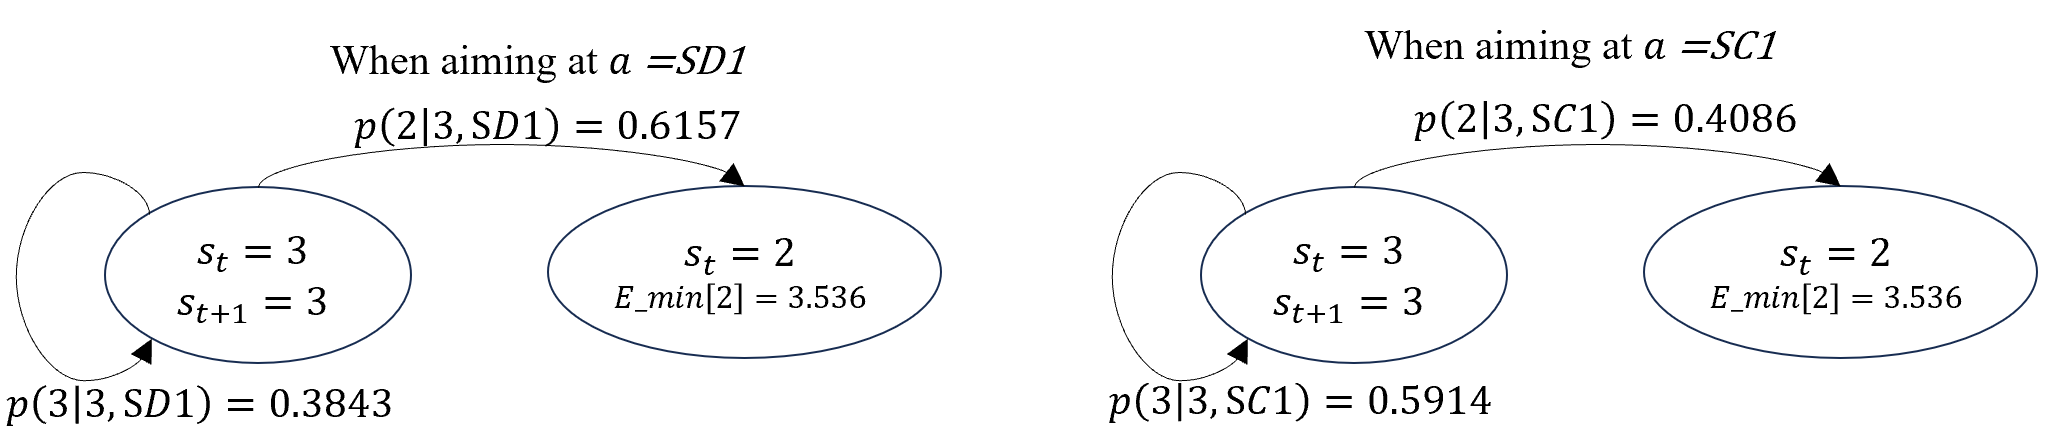
\includegraphics[width=0.60\textwidth]{7.png} 
    \caption{\textbf{Transition diagrams
for a player in state $st = 3$ aiming at two targets}}
    \label{fig:dartboard}
\end{figure}

From the diagram above, it can be determined that the player's optimal decision at $s_t = 3$ is $\text{SD1}$,with $E_{\min}[3] = 5.16$.

\begin{figure}[h]
    \centering
    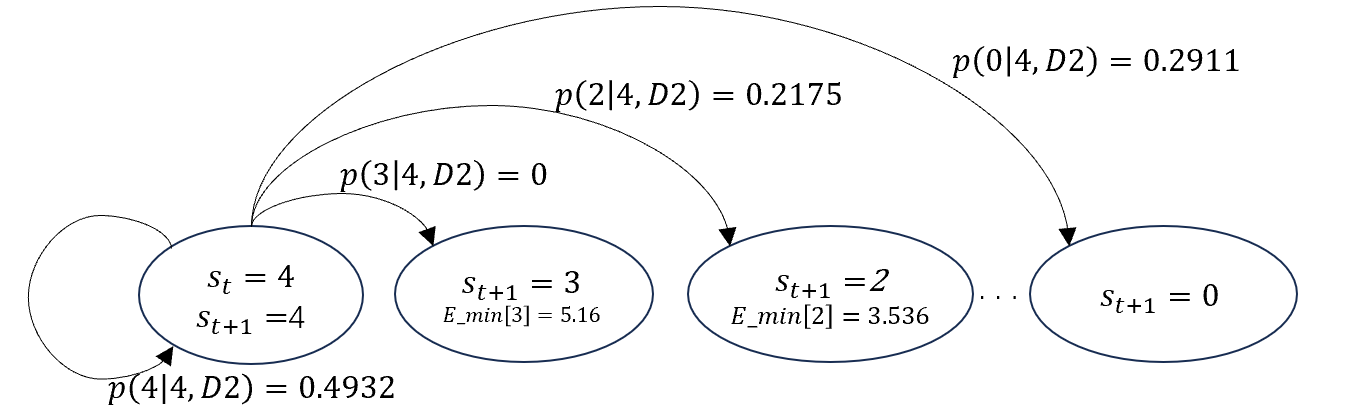
\includegraphics[width=0.60\textwidth]{8.png} 
    \caption{\textbf{Transition diagramsfor a player in state st = 4 aiming at D2}}
    \label{fig:dartboard}
\end{figure}

From the diagram above, it can be determined that the player's optimal decision at $s_t = 4$ is D2,with $E_{\min}[4] = 3.478$. By repeating the process, we can retrospectively calculate the expected number of throws required for the player to complete a 501 game while employing the optimal strategy. Using the data for world champion Michael, a trial calculation yields an expected value of 14.5 throws for completing the game under the optimal strategy. This closely approximates his actual number of throws for game completion. Applying the same method to estimate the throws for Grandma Wang, a high-performing elderly player within the community, reveals an expected value of 71 throws for completing the game under the optimal strategy. This implies that even with consistent performance and sustained stamina throughout the game, Grandma Wang would require approximately 71 throws to complete the 501 games.

\subsection{Game Rule Optimization}

The calculations in the preceding section demonstrate that even a relatively skilled player within the community, such as Grandma Wang, faces considerable difficulty in completing a 501 game. Evidently, the four game rules outlined in Section 3.1 present a significant challenge for the elderly. Therefore, this section explores adjustments to these rules aimed at facilitating successful completion of the 501 games by older players. The specific modifications are detailed below.

\text{\textbf{New Rule 1:}}The final dart no longer requires a "double out." The game is completed when the score is reduced to exactly 0.

\text{\textbf{New Rule 2:}}The game is completed when the score is reduced to 0 or a negative value. It is not necessary to reduce the score to exactly 0.

For \textbf{New Rule 1}, the state space S of the Dart-MDP needs to incorporate new states arising from the rule modification, resulting in $S = {501, 500, 499, ···,2, 1, 0}$. When constructing the state transition diagram, the "double out" restriction is removed. Employing the method described in Section 4.1, we can calculate that Grandma Wang requires 44.17 throws and world champion Michael requires 13.8 throws to complete the game under this new rule.

For\textbf{ New Rule 2}, the player simply needs to greedily select the location with the highest expected score at each throw. The optimal decision for each state is:

\begin{equation}
a^* = \arg\max_{a \in A} \sum_{s_{t+1}} p(s_{t+1} \mid s_t, a) (s_t - s_{t+1})
\tag{8}
\end{equation}

Combining the estimation of dart throwing accuracy for the four older adults and the world champion, as detailed in Section 3.4, we can calculate the optimal target location that maximizes the expected score for a single throw for each older adult. By selecting their respective optimal targets, these individuals can achieve faster game completion, as illustrated in the following table.

\begin{table}[h]
    \centering
    \begin{tabular}{|l|c|c|c|c|c|}
        \hline
        \textbf{Player} & \textbf{Robot} & $\boldsymbol{\sigma_X}$ & $\boldsymbol{\sigma_Y}$ & \textbf{Target} & \textbf{Expected Score} \\
        \hline
        Michael V. Gerwen & U534  & 0.9  & 1.4  & T20  & 38.00 \\
        \hline
        Grandpa Ji       & U2998 & 6.2  & 9.6  & SC8  & 13.71 \\
        \hline
        Aunt Feng        & U3503 & 7.8  & 8.6  & DB   & 13.64 \\
        \hline
        Aunt Zhang       & U3900 & 9.0  & 10.0 & DB   & 12.68 \\
        \hline
        Grandma Wang     & U2919 & 6.0  & 8.8  & SC8  & 14.21 \\
        \hline
    \end{tabular}

    \caption{ \textbf{Optimal targets and expected score for world champion Michael van Gerwen and four elderly dart players under New Rule 2}}
   \end{table}

With the adoption of New Rule 2, the number of throws required for Grandma Wang to complete a 501 game is reduced to approximately 35. Even Aunt Zhang, the player with the lowest skill level, can finish the game within about 40 throws. The world champion, Michael, requires approximately 13 throws to complete the game. This demonstrates that while the rule modification has a negligible impact on high-level players, it significantly lowers the barrier to entry for the elderly participating in this sport.

The experimental data presented above indicate that elderly can select appropriate game rules based on their skill level when participating in darts. Initially, when first engaging in the sport, adopting New Rule 2 is more aligned with practical considerations. As practice frequency increases and skill level gradually improves, New Rule 1 can be incorporated. This approach facilitates a smoother learning curve for the elderly. Once the older players' skill levels, as reflected by their standard deviations in the X and Y directions, reach approximately 4.0, these modified rules can be discarded, allowing them to compete alongside professional players.

\subsection{Training Strategy Optimization}
Observation of world champion Michael's performance in competitions reveals that his accuracy when aiming for T20 surpasses that of other high-scoring targets such as T19 and T18. This is attributed to the fact that high-level players dedicate more practice time to T20, the highest-scoring target, during training. Prior to official matches, these players also select a few specific targets for warm-up rather than practicing on all targets. Drawing upon these practices of high-level players, we now explore training strategies for the elderly players.

\textbf{Training Model Assumption}: Within a given timeframe, after a player practices aiming at a specific target location $a \in A$ on the dartboard a certain number of times, the standard deviations $(\sigma_X, \sigma_Y)$ for throws towards this location will decrease by a certain percentage, while those for other locations remain unchanged.

\textbf{Problem Statement}:Which target, when subjected to intensified practice, can contribute to enhancing this player's performance in the 501 games?

Based on the previous estimation results, Grandma Wang's overall skill level is characterized by standard deviations of 6.0 and 8.8 in the X and Y directions, respectively. Let us assume that after a period of intensive training, Grandma Wang's standard deviations when aiming at a specific location $a \in A$ are reduced by $20\%$,resulting in $(\sigma_X = 4.8, \sigma_Y = 7.0)$,while accuracy at other locations remains unchanged. Applying the methodology for New Rule 1 and conducting trials across all targets on the dartboard, we obtain the following results:

\begin{table}[H]
\centering
\begin{minipage}{0.6\textwidth} 
    \begin{tabular}{|p{1cm}|p{2cm}|p{2cm}|} 
    \hline
    \textbf{Target for Practice} & \textbf{Expectation of the Minimum Number of Throws} & \textbf{Decrease in the Number of Throws} \\
    \hline
        SC8  & 41.7 & 2.4 \\
        SC11 & 41.8 & 2.4 \\
        SC16 & 42.2 & 2.0 \\
        SC7  & 42.4 & 1.8 \\
        SC14 & 43.0 & 1.2 \\
        T11  & 43.1 & 1.1 \\
        SC19 & 43.2 & 1.0 \\
        T19  & 43.8 & 0.4 \\
        T18  & 44.0 & 0.2 \\
        T20  & 44.0 & 0.1 \\
        DB   & 44.1 & 0.0 \\
    \hline
    \end{tabular}
    \caption{\textbf{Optimal practice targets that can most effectively reduce the number of throws for Grandma Wang}}
\end{minipage}
\hspace{1cm} 
\begin{minipage}{0.3\textwidth} 
    \centering
    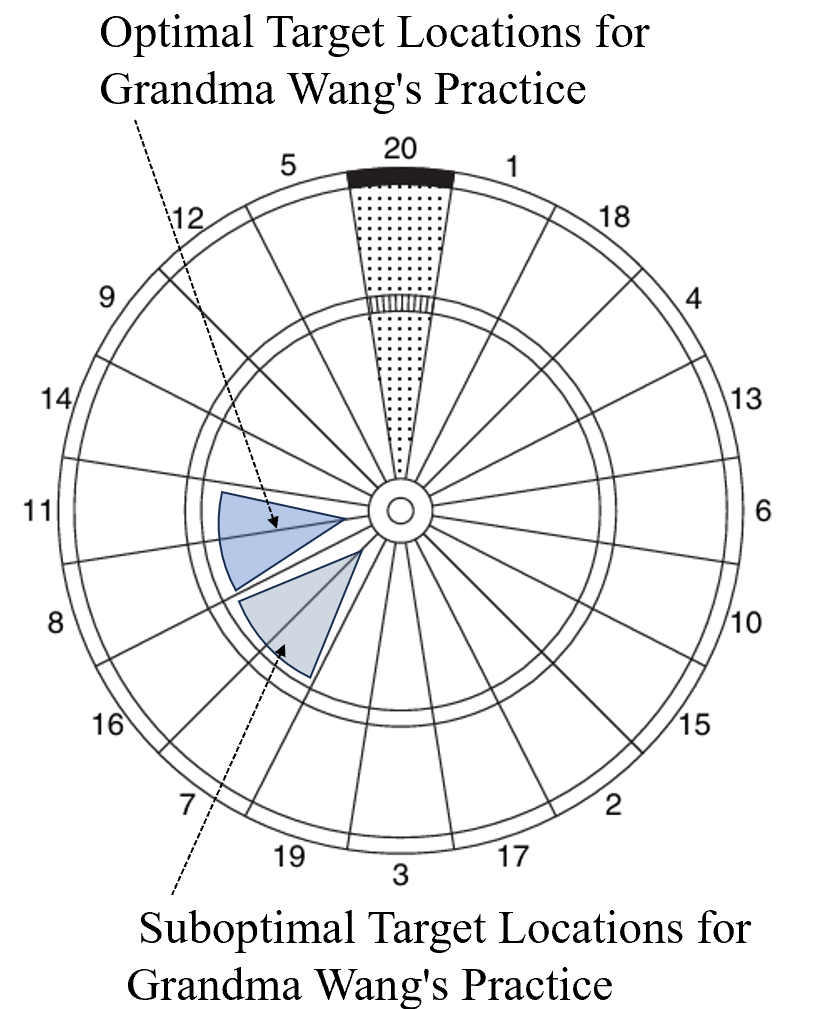
\includegraphics[width=\textwidth]{example.png} 
\end{minipage}
\end{table}

From the table above, it is evident that practicing on all locations does not uniformly contribute to improving Grandma Wang's performance in 501 games. Intensive practice on high-scoring targets such as T20, T19, T18, and DB yields negligible improvement. Instead, selecting positions like SC8 and SC11 for practice, and leveraging these positions during the game, proves to be more beneficial. Even if her throws are not entirely accurate, darts landing in adjacent regions still yield relatively high scores, thus effectively enhancing her overall performance.

\section{Conclusion}

This research originated from the darts society at Beijing No.101 High School, where practical difficulties were encountered in promoting dart-based fitness activities for the elderly within the local communities. To quantitatively measure and analyze these challenges, this study established a dart throwing strategy model based on the MDP. Utilizing dart throwing data collected during these activities, the nearest neighbor method was employed to estimate the throwing accuracy of the elder participants. Subsequently, the transition probabilities of the Markov process within the model were solved using the polar coordinate form of the bivariate normal distribution. Building upon this model, we propose three optimization strategies for the elderly engaging in darts: the first strategy assists older adults in selecting the most rational throwing targets in the 501 games; the second strategy guides the elderly in adopting game rules suitable for their skill levels; and third strategy aids in formulating reasonable training plans. These three strategies collectively aim to facilitate a smooth transition through the initial learning phase of darts for the elderly, encouraging their long-term participation in the sport.

\text During dart promotional events held within the local communities, members of the darts society observed that the sport is also highly accessible to individuals requiring greater care in our society, such as those reliant on wheelchairs or confined to bed rest. The strategies proposed in this study are also applicable and beneficial to these groups, enabling them to participate in and derive enjoyment form the sport.


\begin{center}
\section*{\large Appendix}
\end{center}

\begin{itemize}
    \item \textbf{Calculating the aiming points (Centroids) for all target areas on a dartboard.}
\end{itemize}

The coordinates $(\mu_{a_X}, \mu_{a_Y})$ of the aiming point (centroid) for each target area (annular sector) can be calculated using the centroid formula for an annular sector. The centroid lies on the bisector of the sector angle, and its distance from the center of the dartboard is as follows:


\begin{figure}[h]
\begin{minipage}{0.5\textwidth}
    \begin{align*}
    l &= \frac{4 \sin\left(\frac{\theta}{2}\right) \left( r_2^3 - r_1^3 \right)}{3 \theta \left( r_2^2 - r_1^2 \right)}
    \end{align*}
\end{minipage}
\begin{minipage}{0.5\textwidth} 
    \centering
    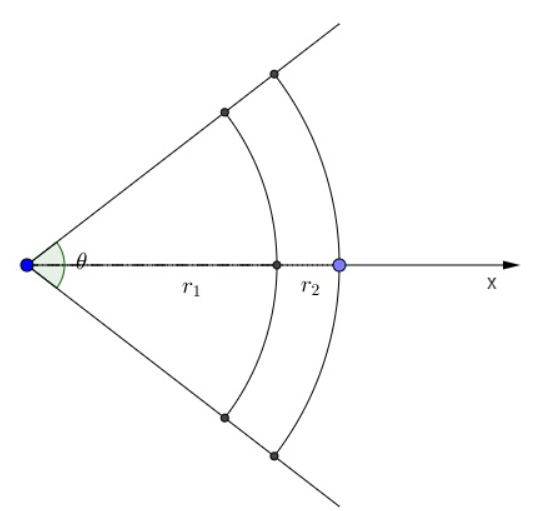
\includegraphics[width=\textwidth]{9.png}
\end{minipage}
\caption{\textbf{Calculating the centroid of an annular sector in the dartboard}}
\end{figure}

\begin{itemize}
    \item \textbf{Example of transition probability solving.}
\end{itemize}

\text A player's skill level is characterized by the standard deviations
$(\sigma_X, \sigma_Y)$ of two independent bivariate normal distributions in the X and Y directions. When a player aims at ${\text{target}} = a$ and hits a specific area $\text{hit} = h$,the probability of this event can be expressed using the integral formula of the bivariate normal distribution, where $(\mu a_X, \mu a_Y)$ represent the coordinates of the centroid of the $\text{target} = a$.

$$P(\text{target} = a, \text{hit} = h) = \iint_h \frac{1}{2 \pi \sigma_X \sigma_Y} \exp\left( - \frac{(\rho \cos \theta - \mu a_X)^2}{2 \sigma_X^2} - \frac{(\rho \sin \theta - \mu a_Y)^2}{2 \sigma_Y^2} \right) \rho \, d\rho \, d\theta$$

\begin{figure}[H]
    \centering
    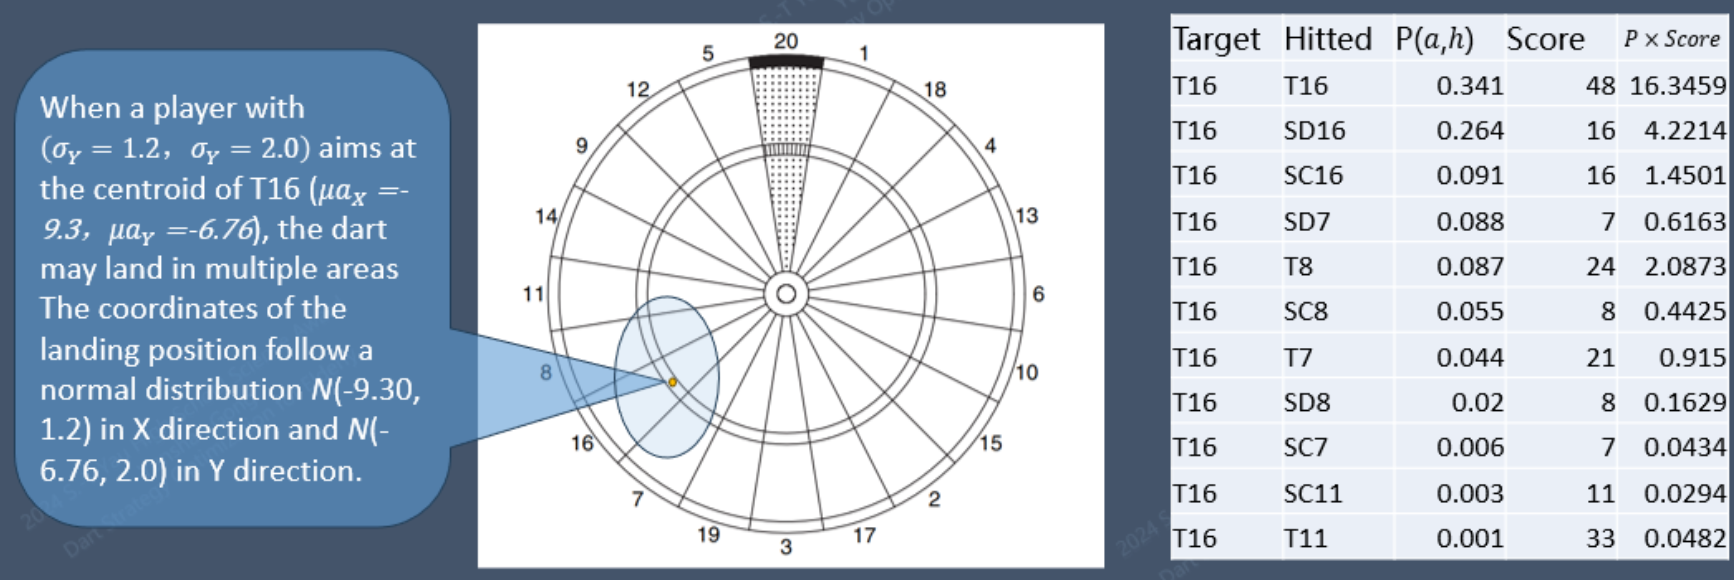
\includegraphics[width=0.60\textwidth]{10.png} 
    \caption{\textbf{An example of solving the transition probability
of the MDP}}
    \label{fig:dartboard}
\end{figure}

\begin{itemize}
    \item \textbf{A bug report concerning an anomaly in the calculation of double integrals was submitted to the maintainer of the relevant R package, and a reply from the package author was received.}
\end{itemize}

\text The extensive computation of double integrals required for this research encountered issues with abnormal program termination when using R. To address this, a bug report documenting these instances was submitted to the R development team. The package author acknowledged our report and proposed fixes, but stated that they do not intend to update the library further.

\begin{figure}[H]
    \centering
    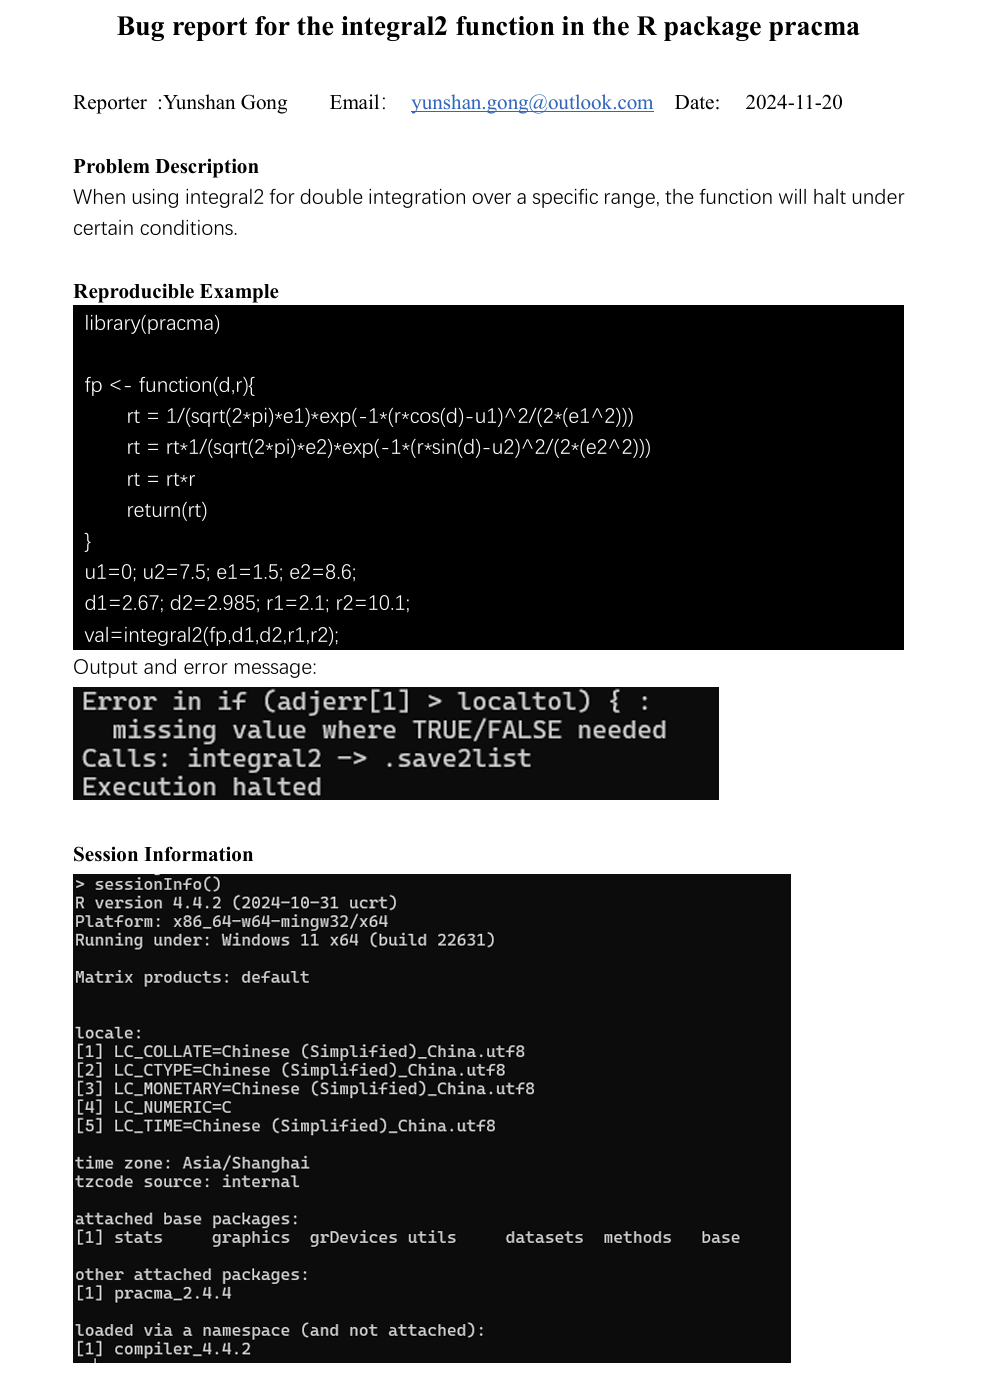
\includegraphics[width=0.60\textwidth]{11.png} 
    \caption{\textbf{Bug Report for the intintegral 2 function in the R package pracma}}
    \label{fig:dartboard}
\end{figure}

\begin{figure}[H]
    \centering
    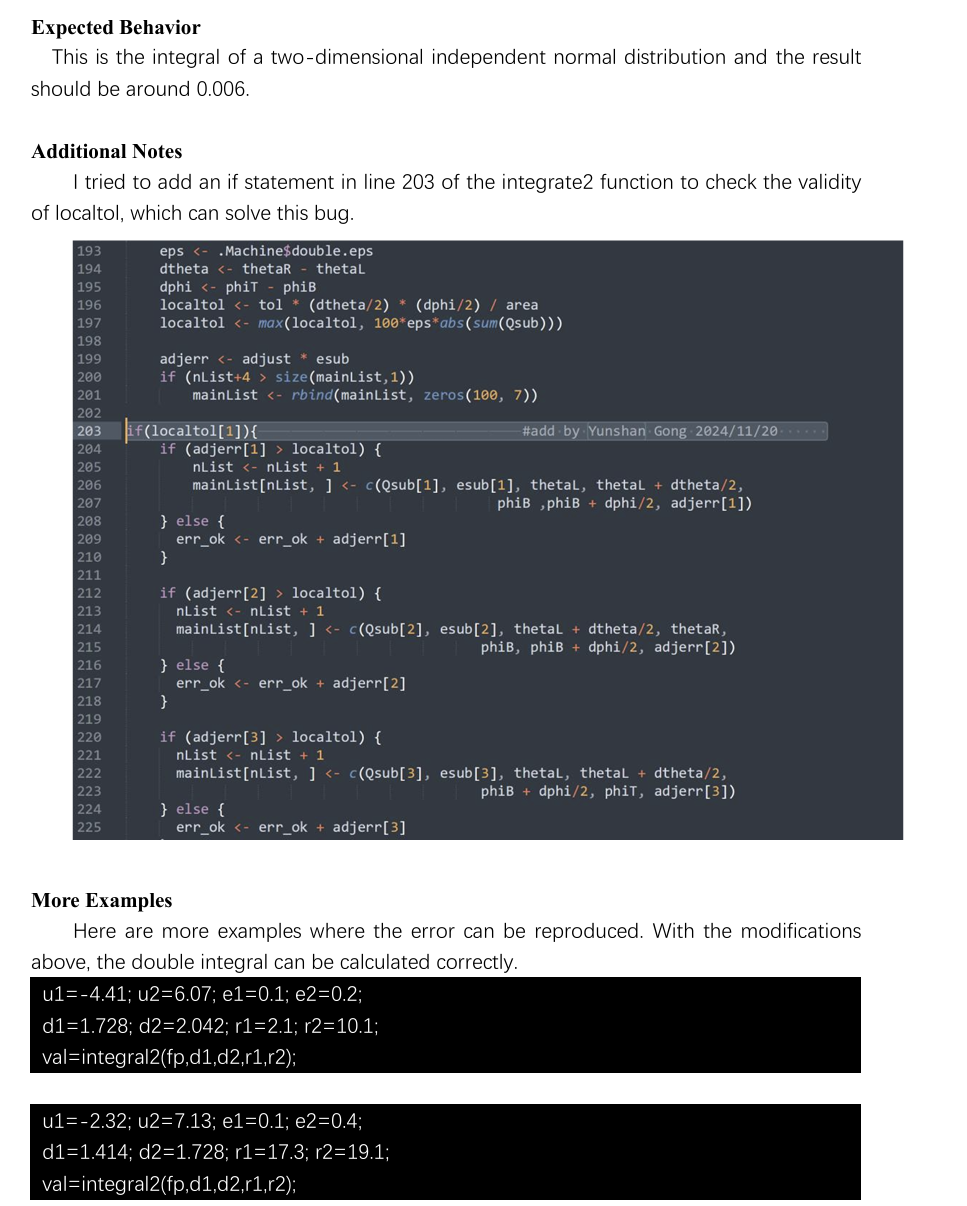
\includegraphics[width=0.60\textwidth]{12.png} 
    \caption{\textbf{Bug Report for the intintegral 2 function in the R package pracma}}
    \label{fig:dartboard}
\end{figure}

\begin{itemize}
    \item \textbf{Using SQLite Studio to store and manage throwing data for robots, professional Players, and elderly Players.} 
\end{itemize} 

\text The database contains three tables: the Expert table stores data for professional players from the 2019 Masters tournament, the robots table stores simulated data for dart-throwing robots, and the Sample table stores throwing data for elderly players. To facilitate the observation and analysis of this data, a series of queries has been constructed, as shown in the lower left panel. The data in the right panel displays the robots ranked in order of their similarity to Ms. Wang's skill level, as determined by the nearest neighbor method.

\begin{figure}[H]
    \centering
    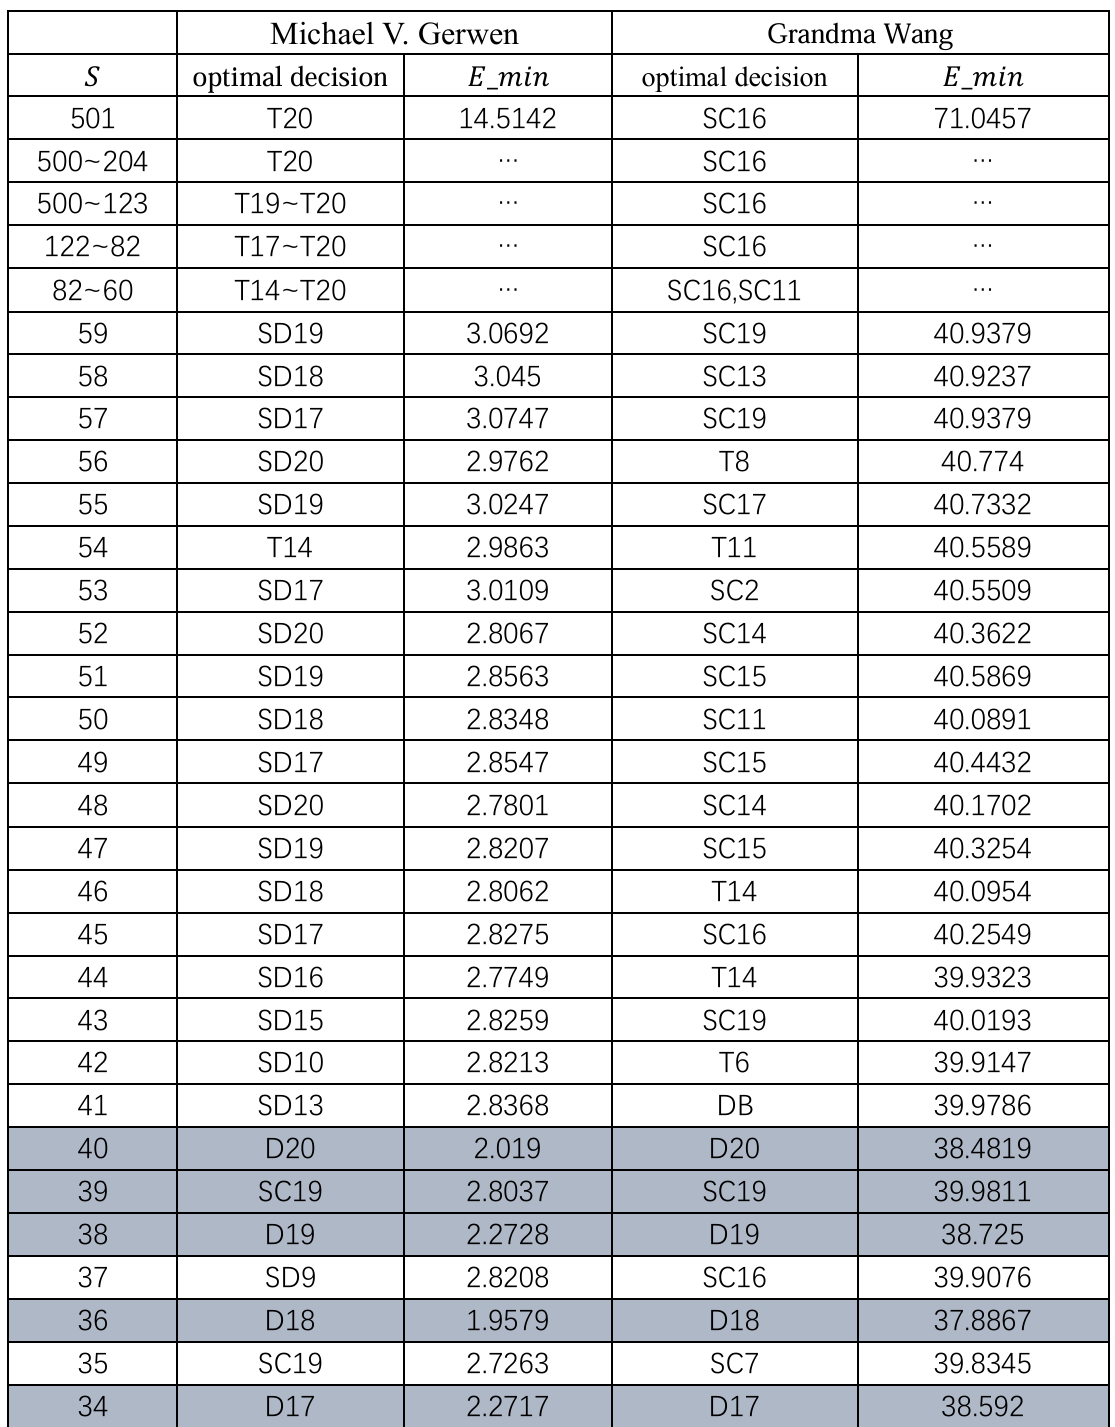
\includegraphics[width=0.60\textwidth]{13.png} 
    \caption{\textbf{Bug Report for the intintegral 2 function in the R package pracma}}
    \label{fig:13}
\end{figure}
\newpage
\begin{itemize}
    \item \textbf{Comparison of optimal strategies for completing a 501 dart game: world champion Michael vs. Grandma Wang from Local Community.}
\end{itemize}

\text In the following table, shaded areas indicate states where both players adopt the same decision. It is evident that the optimal strategies for different players in the game vary significantly, with convergence to identical decisions occurring only in the final stages of the game.   

\begin{figure}[H]
    \centering
    \begin{minipage}{0.45\textwidth}  
        \centering
        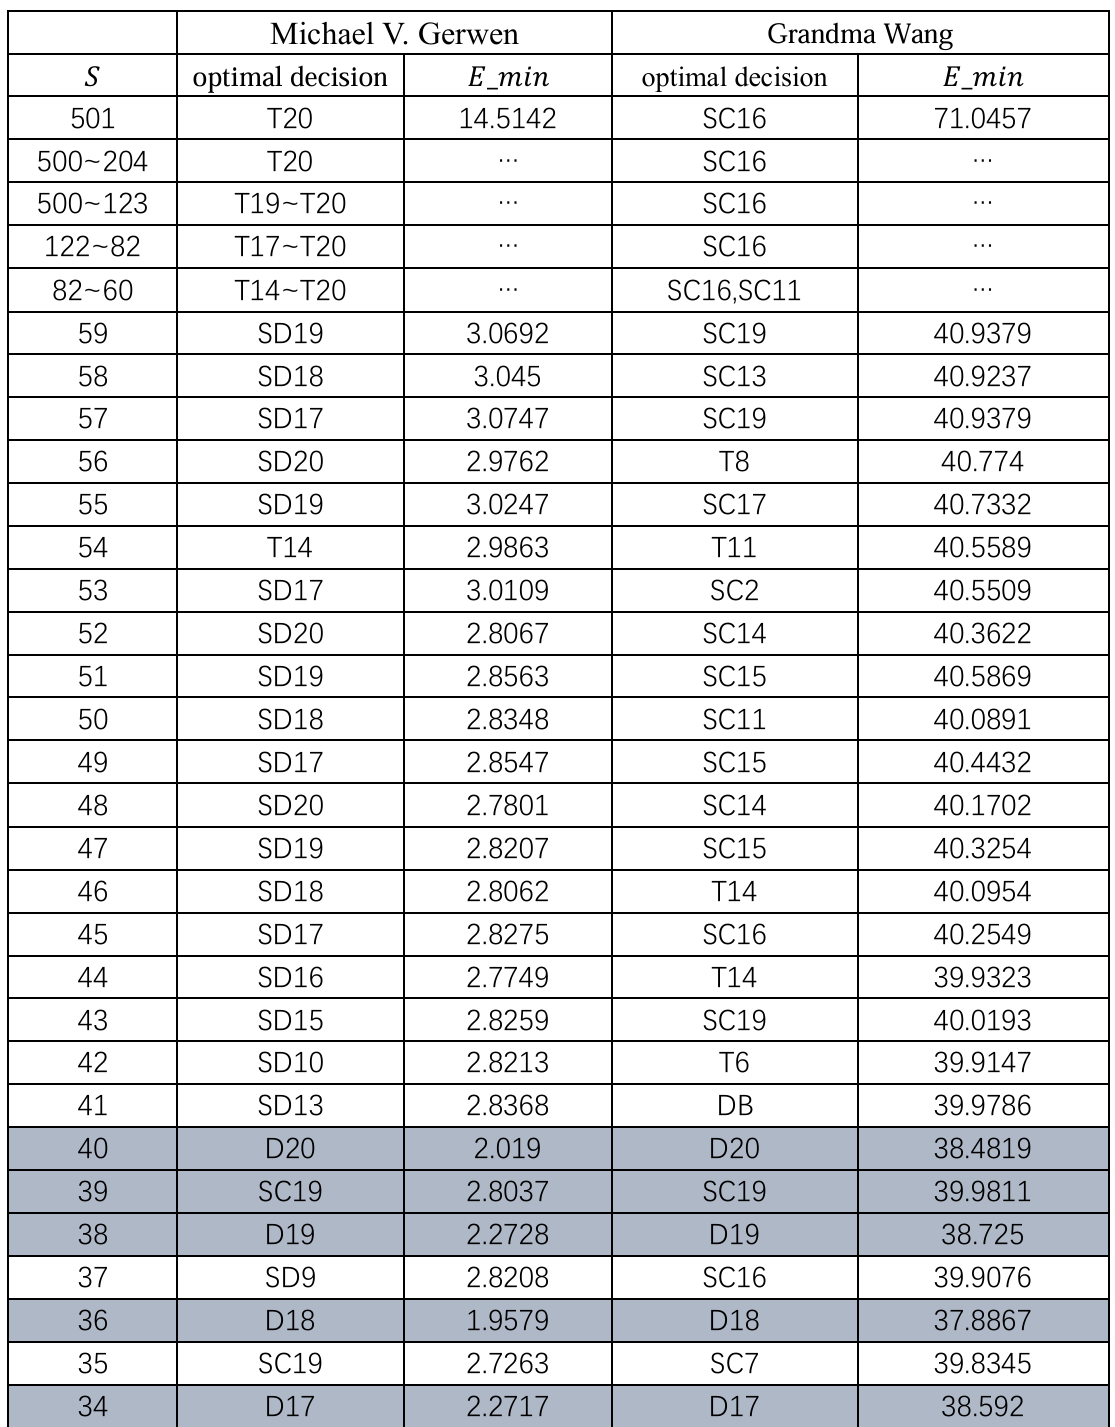
\includegraphics[width=\textwidth]{picture1.png}  
        \caption{\textbf{Comparison of optimal strategies of the two players}}  
        \label{fig:image1}
    \end{minipage} \hspace{0.5cm} 
    \begin{minipage}{0.45\textwidth} 
        \centering
        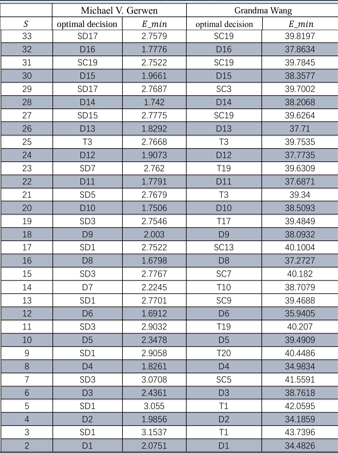
\includegraphics[width=\textwidth]{picture2.png} 
        \caption{\textbf{Comparison of optimal strategies of the two players}}  
        \label{fig:image2}
    \end{minipage}
\end{figure}

\newpage
\begin{itemize}
    \item \textbf{The Darts society from Beijing No. 101 High School hosted dart events for the elderly in local communities.}
\end{itemize}

\text The darts society promoted the sport of darts to older adults within the local communities, while simultaneously conducting interviews, surveys, and data collection to assist these individuals in maintaining long-term engagement with the sport.
\begin{figure}[H]
    \centering
    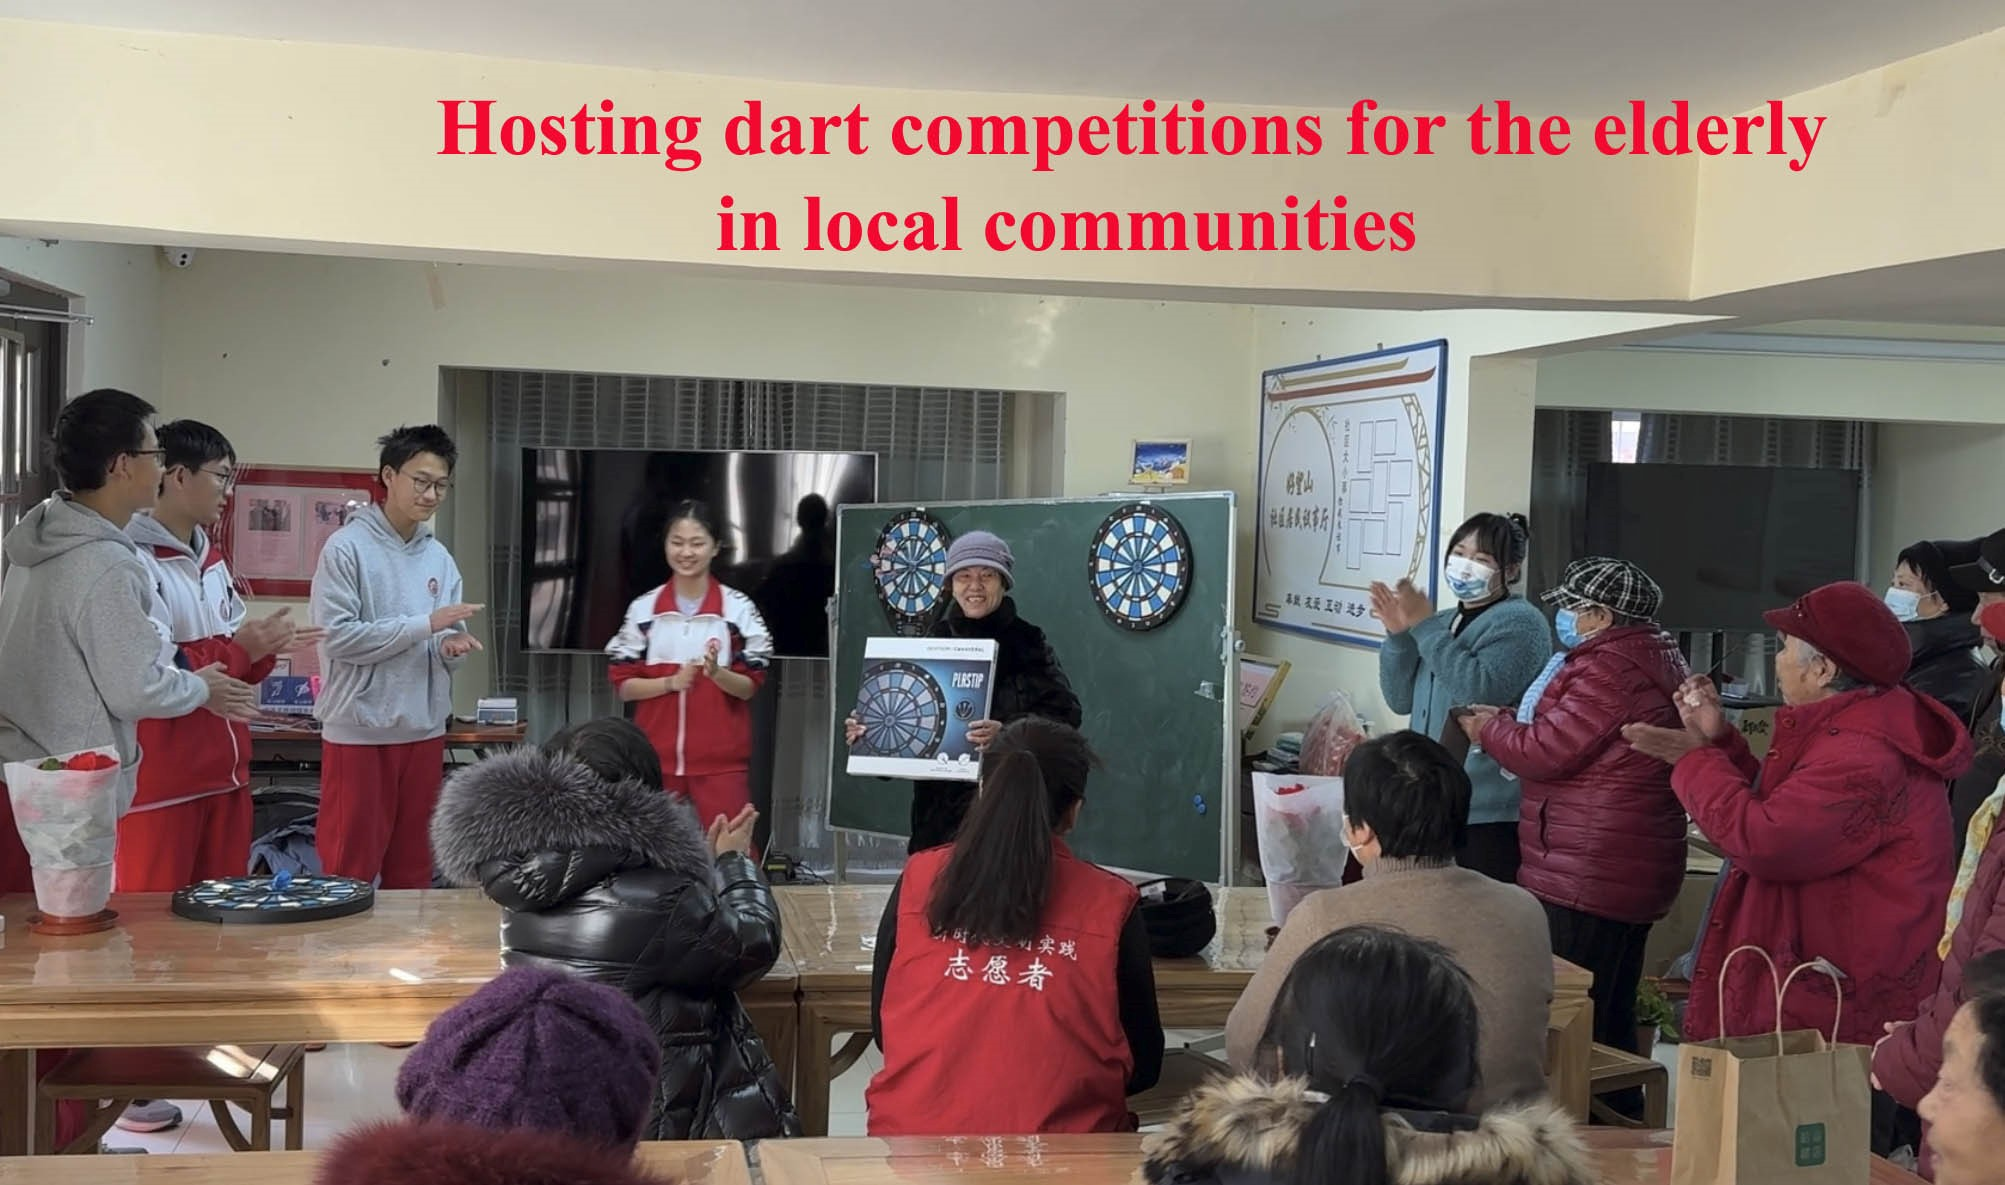
\includegraphics[width=0.60\textwidth]{14.jpg} 
    \caption{\textbf{Hosting dart competitions for the elderly in local communities}}
    \label{fig:dartboard}
\end{figure}


\section*{Acknowledgement}
\text In January 2024, I participated in a writing competition hosted by the Association for Women in Mathematics (AWM), focusing on the theme of women's power in mathematics. I had the fortunate opportunity to interview Professor Qi Qi, through which I learned about her research applying game theory to optimize public housing allocation mechanisms in Hong Kong, to support low-income and vulnerable groups.

This interview profoundly affected me, revealing the potential of academic knowledge to make a real difference in the lives of others and contribute to a better world. Consequently, this experience inspired me to apply mathematical thinking to real-world issues. I continued to learn from Professor Qi after the interview, gaining both knowledge and confidence from our interactions.

The research stems from the Darts Society at Beijing No.101 High School, where I serve as the president. The society was initially established to help classmates alleviate academic stress and protect their eyesight. Through our activities, we observed that this sport is particularly well-suited for the elderly, especially those with limited mobility, and darts offers a rare opportunity for this demographic to participate in sports.
Consequently, our society actively promotes the sport to older adults within local communities and neighborhoods, and we collected data throughout these activities.

In early July 2024, I presented the activities and dataset of the society to Professor Qi. Upon hearing my presentation, Professor Qi responded positively to my presentation, recognizing the value of exploring the connection between darts and older adults within the context of today's aging society. After offering encouragement, Professor Qi astutely pointed out that the progression of a 501 game constitutes a sequential decision-making process, amenable to quantitative analysis using Markov-related tools. Following this direction, I acquired the book "Markov Decision Process Theory and Applications" during the summer of 2024. With the aid of this book, I was intrigued to discover how effectively the five elements of the Markov Decision Process could model the dart games. Under Professor Qi’s mentorship, I progressively developed the main framework of this research over the summer and documented it in written form. Throughout the writing process, Professor Qi diligently guided me on the norms and techniques of academic writing.

The members of the Darts Society at Beijing No.101 High School provided invaluable support and assistance to this research. Together, we hosted dart events for the elderly, accumulated data, designed posters, and engaged in brainstorming sessions. We even devised a dart game adapted for visually impaired individuals. I extend my sincere gratitude to all members of our darts society.

Finally, I express my appreciation to Beijing No.101 High School for providing not only an excellent learning environment and ample space for society activities but also the opportunity to participate in the advanced mathematics placement test upon enrollment. This enabled me to systematically study calculus in my first year of high school and to enroll in the school's mathematical modeling course. Through these two courses, I acquired fundamental data processing and modeling skills, laying the groundwork for this research.

Professor Qi Qi's guidance was entirely voluntary, provided without any form of compensation. Here, I would like to express my heartfelt gratitude for her dedicated mentorship. She not only taught me how to conduct research, but also how to do research with compassion and empathy. 

\begin{thebibliography}{9}

\bibitem{ref1}
Department of Aging and Health, National Health Commission of the People's Republic of China, "'14th Five-Year Plan' for Healthy Aging," Mar. 01, 2022. \url{http://www.nhc.gov.cn/lljks/pqt/202203/c51403dce9f24f5882abe13962732919.shtml}.

\bibitem{ref2}
I. K. Crombie, "Why older people do not participate in leisure time physical activity: a survey of activity levels, beliefs and deterrents," \textit{Age and Ageing}, vol. 33, no. 3, pp. 287–292, May 2004, doi: \url{https://doi.org/10.1093/ageing/afh089}.

\bibitem{ref3}
M. Takeda, N. Yasuda, S. Ito, and M. Abe, "Effects of Habitual Darts Training on Cognitive Function in Elderly People," \textit{The Harris Science Review of Doshisha University}, vol. 58, no. 2, Jul. 2017.

\bibitem{ref4}
Xiao Xin, "Throwing darts to practice balance," \textit{Friends of the Seniors}, vol. 17, no. 58, 2013.

\bibitem{ref5}
"Improve coordination by playing darts," \textit{Family Medicine}, vol. 5, no. 29, 2019.

\bibitem{ref6}
R. J. Tibshirani, A. Price, and J. Taylor, "A statistician plays darts," \textit{Journal of the Royal Statistical Society: Series A (Statistics in Society)}, vol. 174, no. 1, pp. 213–226, Jul. 2010, doi: \url{https://doi.org/10.1111/j.1467-985x.2010.00651.x}.

\bibitem{ref7}
M. B. Haugh and C. Wang, "Play Like the Pros? Solving the Game of Darts as a Dynamic Zero-Sum Game," \textit{INFORMS Journal on Computing}, Apr. 2022, doi: \url{https://doi.org/10.1287/ijoc.2022.1197}.

\bibitem{ref8}
D. James and J. Potts, "Experimental validation of dynamic stability analysis applied to dart flight," \textit{Sports Engineering}, vol. 21, no. 4, pp. 347–358, Jun. 2018, doi: \url{https://doi.org/10.1007/s12283-018-0279-9}.

\end{thebibliography}
\end{document}
